\documentclass[solutionsatend]{ouunit}
% Class options available
% final = remove drafting features for final output (eg date/time in footer)
% solutionsatend = move exercise and activity solutions to location of \printexercisesolutions
% twocolumnsolutions = typeset \printexercisesolutions and \printactivitysolutions in two columns
% reduceda4 = change paper size to reduced a4
% previewonly = produce quick preview representation for yap (pk fonts)

\usepackage[nopar]{lipsum}%just for this example
\usepackage{outikz}% the ouunit.sty is compatible with the OU figure styles

%metadata
\modulecode{Mxxx}
\moduletitle{Generic module}
\unitid{0}
\unittitle{Style test}
\draftno{D1}
\author{Robert Hasson}

%local definitions for this unit

%lower resolution logo for smaller files
\DeclareRobustCommand{\oulogo}{
\includegraphics[width=3.5cm]{ou_compact_cmyk_24mm}}

%friendly names for box styles
\newenvironment{highlight}[1][]{\begin{style2box}[#1]}{\end{style2box}}

%Example of setting up a theorem as a boxed style
\newcounter{theorem}
\newenvironment{theorem}[1][]{\refstepcounter{theorem}\begin{style2box}[Theorem \thetheorem\quad #1]}{\end{style2box}}
\newenvironment{theorem*}[1][]{\begin{style2box}[Theorem\quad #1]}{\end{style2box}}

\DeclareRobustCommand{\hexagon}{\tikz{\draw[thin] (0:0.15) -- (60:0.15) -- (120:0.15) -- (180:0.15) -- (240:0.15) -- (300:0.15) --cycle;}}

\begin{document}
\makefrontpages
\introduction
\lipsum[133]
\[
E=mc^2
\]
\lipsum[133]
\section{Headings}
\lipsum[133]
\subsection{OnePointOne}
\lipsum[133]
\subsubsection{OnePointOnePointOne}
\lipsum[133]
\paragraph{Titledparagraph style -- same page on VLE}
\lipsum[133]
\section{Margin notes}
\begin{highlight}
\lipsum[133]
\marginnote{Hello}

\lipsum[133]
\marginnote{Hello}
\[
E=mc^2\marginnote{Hello}
\]
\end{highlight}
\lipsum[133]
\begin{highlight}
\lipsum[133]
\marginnote{Hello}
\end{highlight}
\begin{align*}
y &=x\\
&=1\marginnote{alongside the 1.}\\
&=2\\
&=3
\end{align*}
Note the large space above the aligned equations, when they immediately follow a box.
\begin{highlight}[Title]
\lipsum[133]
\marginnote{Hello}
\end{highlight}
\section{Boxes}
The generic box styles exist, but authors should use context names (such as `highlight', `history' or `aside' rather than using the generic box styles directly. All boxes break between pages automatically.\index{boxes}
\begin{style1box}[Box title style1box]
\lipsum[1]
\end{style1box}
\begin{style2box}[Box title style2box]
\lipsum[2]
\end{style2box}
\begin{style3box}[Box title style3box]
\lipsum[3]
\end{style3box}
\begin{style3box}
\lipsum[3]
\end{style3box}
\begin{style4box}[Box title style4box]
\lipsum[4]
\end{style4box}
The fourth box style changes in the online templates. The online version of the fourth box style is also implemented, just in case documents want to mimic the look of online documents.\index{online box|see{boxes}}
\begin{onlinestyle4box}[Box title online style4box]
\lipsum[4]
\end{onlinestyle4box}
Titled box containing just a list.
\begin{style4box}[Solution]
\begin{enumerate}
\item part 1.
\item part 2.
\item part 3.
\end{enumerate}
\end{style4box}
\section{Lists}
\lipsum[133]
\begin{enumerate}
\item
\lipsum[133]
\item
\lipsum[133]
\end{enumerate}
\lipsum[133]
\begin{enumerate}
\item
\lipsum[133]
\item
\lipsum[133]
\begin{enumerate}
\item
\lipsum[133]
\item
\lipsum[133]
\end{enumerate}
\end{enumerate}
\begin{highlight}
\lipsum[133]
\begin{enumerate}
\item
\lipsum[133]
\item
\lipsum[133]
\begin{enumerate}
\item
\lipsum[133]
\item
\lipsum[133]
\end{enumerate}
\end{enumerate}
\end{highlight}
\lipsum[133]
\begin{description}
\item[First item]
\lipsum[133]
\item[Second item]
\lipsum[133]
\begin{description}
\item[Nested first item]
\lipsum[133]
\item[Nested second item]
\lipsum[133]
\end{description}
\end{description}
\lipsum[133]
\begin{itemize}
\item
\lipsum[133]
\item
\lipsum[133]
\begin{itemize}
\item
\lipsum[133]
\item
\lipsum[133]
\end{itemize}
\end{itemize}
\lipsum[133]
\section{Equations}
Unnumbered equations: use \verb”\[” and \verb”\]” such as
\[
E=mc^2
\]
Note that \verb”\\” is not allowed within displayed equations. Use \verb"align*" instead, e.g.
\begin{align*}
&\text{first line}\\
&\text{second line}
\end{align*}
Fot numbered equations use the \verb”equation” (the OUTeX command \verb”\donumber” is not defined).
\begin{equation}
\text{equation }1
\end{equation}
For aligned equations use \verb”align*”
\begin{align*}
a& =b\\
&=c
\end{align*}
For numbered aligned equations use \verb”align”
\begin{align}
a& =b\label{eqn-line1}\\
&=c\label{eqn-line2}
\end{align}
Reference to line one, equation~(\ref{eqn-line1}), and to line two equation~(\ref{eqn-line2}).

To number only one line use \verb”\nonumber”
\begin{align}
a& =b\nonumber\\
&=c\label{eqn-middle-line}\\
&=d\nonumber
\end{align}
Compare spacing with display math
\[
y=x^2
\]
Matrix with no arguments (as AMSmath standard, defaults to cccccc) and matrix with optional placement arguments.
\[
\begin{pmatrix}
1 & -2\\
-3 & 4
\end{pmatrix}
\qquad
\begin{pmatrix}[r|r]
1 & -2\\
-3 & 4
\end{pmatrix}
\]

\section{Exercises, Activities and Examples}

\lipsum[133]

\lipsum[134]

\begin{exercise}
\label{exe-fred}
This is a question
\begin{enumerate}
\item First part
\item Second part
\end{enumerate}
\begin{solution}
This is the answer.
\begin{enumerate}
\item First part answer
\item Second part answer
\begin{equation}
\text{equation in solution} \label{eqn-sol1}
\end{equation}
Testing verbatim in moving solution \verb"hello".

Testing reference to equation in solution, namely equation~\ref{eqn-sol1}.
\end{enumerate}
\end{solution}
\noendrule
\end{exercise}
\begin{exercise}[second exercise in exercises with title]
\lipsum[133]
\begin{solution}
\lipsum[133]
\end{solution}
\noendrule
\end{exercise}
\begin{exercise}[third exercise in exercises with a very very long title]
\lipsum[133]\icons{web}{}{}
\begin{solution}
\lipsum[133]
\end{solution}
\end{exercise}
That was Exercise~\ref{exe-fred}, which contained equation~\ref{eqn-sol1}.
\begin{equation}
2
\end{equation}
Here we tell students about margin icons, such as the one alongside in the margin.\icons{web}{}{} The following exercise has some icons in the margin. For drafting these are just some text in a box. With the final option they will be the standard set of icons.

\begin{exercise}[\icons{calc}{web}{}]\label{exe-jim}
This is another question
\begin{solution}
This is another answer.
\end{solution}
\end{exercise}
That was Exercise~\ref{exe-jim}. 


The following exercise shows the style to use instead of the OUTeX command \verb”\intertext”.
\begin{exercise}[Intertext style question]\label{exe-intertext}
This is another question
\begin{enumerate}
\item Part one.
\item Part two.
\end{enumerate}
Here are futher instructions.
\begin{enumerate}[resume]
\item Part three.
\item Part four.
\end{enumerate}
\begin{solution}
\begin{enumerate}
\item Solution one.
\item Solution two.
\item Solution three.
\item Solution four.
\end{enumerate}
\end{solution}
\end{exercise}

\makeatletter
%
\makeatother

The following exercise with inline parts
\begin{exercise}[inline question]\label{exe-intertext2}
This is another question
\begin{enumerate}
\item Part one.
\item Part two.
\begin{enumerate*}
\item Part one.
\item Part two.
\item Part three.\newline
\item Part four.
\end{enumerate*}
\item Part three.
\item Part four.
\end{enumerate}
\begin{solution}
\begin{enumerate}
\item Solution one.
\item Solution two.
\begin{enumerate}
\item Part one.
\item Part two.
\item Part three.
\item Part four.
\end{enumerate}
\item Solution three.
\item Solution four.
\end{enumerate}
\end{solution}
\end{exercise}


\lipsum[2]
\begin{example}
\lipsum[133]
\begin{solution}
\lipsum[133]
\end{solution}
\end{example}
\lipsum[133]
\begin{activity}[Using activities]
\lipsum[133]

Note the use of \verb”\noendrule” to suppress the rule between activities.
\begin{solution}
\lipsum[133]
\end{solution}
\noendrule
\end{activity}
\begin{activity}[Another activity\icons{web}{}{}]
\lipsum[133]
\begin{solution}
\lipsum[133]
\end{solution}
\end{activity}

Now for an exercise with inline options
\begin{exercise}
Here is a question with inline options. Plot the following graphs.
\begin{enumerate*}
\item $y=x^2$
\item $y=\sin(x)$
\item $y=x^2$
\item $y=\sin(x)$
\item $y=x^2$
\item $y=\sin(x)$
\item $y=x^2$
\item $y=\sin(x)$
\end{enumerate*}
\end{exercise}



\section{Tables and figures}

\lipsum[133]

\begin{table}
\caption{Caption\label{tab-test}}
\begin{tabular}{|l|l|}
\hline
 Hello & World\\
\hline
\end{tabular}
\end{table}

This is a reference to Table~\ref{tab-test}.

\lipsum[133]
\begin{table*}
\begin{tabular}{ll}
 Hello & World\marginnote{plain table with no number or caption.}\\
\end{tabular}
\end{table*}
\lipsum[133]



\begin{figure}
\caption{Figure test using Tikz}
\label{fig-test-tikz}
\begin{tikzpicture}
\draw[axis] (-0.5,0) -- (4,0) node[xlab]{$x$};
\draw[axis] (0,-0.5) -- (0,4) node[ylab]{$y$};
\draw[red,domain={0:3.5}] plot (\x,{(\x)^2/4}) node[black,right] {$y=x^2$};
\end{tikzpicture}
\end{figure}

This is a reference to Figure~\ref{fig-test-tikz}.

\begin{figure}
\caption{Figure test using includegraphics\label{fig-test-includegraphics}. This figure has an exceedingly long caption so that the justification can be checked. Testing Blah Blah Blah Blah Blah Blah Blah Blah Blah Blah Blah Blah Blah Blah Blah Blah Blah Blah Blah Blah Blah Blah Blah Blah Blah Blah Blah Blah Blah Blah Blah Blah Blah Blah Blah Blah Blah Blah Blah Blah.}
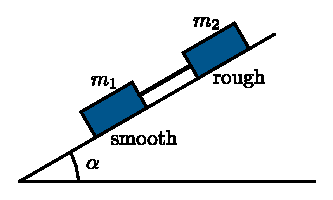
\includegraphics[width=4cm]{test}
\end{figure}

This is a reference to Figure~\ref{fig-test-includegraphics}.

Test for wide figure.

\begin{widefigure}
\caption{Widefigure test\label{fig-test-widefigure-one}}
\begin{tikzpicture}
\draw[axis] (0,0) -- (15,0) node[xlab] {$x$};
\draw[axis] (0,-1.5) -- (0,1.5) node[ylab] {$y$};
\draw (0,0) sin (2,1) cos (4,0) sin (6,-1) cos (8,0) sin (10,1) node[above] {$y=\sin x$} cos (12,0) sin (14,-1);
\end{tikzpicture}
\attrib{\width{100}}%extra OU attributes can be added using an attrib command
\end{widefigure}


\lipsum[134]
\begin{marginfigure*}
\fboxsep 0pt%temporary fix for figurebox
\begin{outikzfig}[figurebox]{margin}
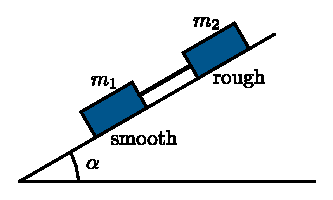
\includegraphics[width=4cm]{test}
\end{outikzfig}
\end{marginfigure*}
\marginnote{Marginfigure* test}[4ex]

\lipsum[133]

\begin{exercise}\label{exe-fig-test}
This is another question
\begin{solution}
Here is a numbered figure:
\begin{figure}
\caption{Figure test \label{fig-placement-test}}

\begin{tikzpicture}
\draw (0,0) -- (1,1);
\draw (1,0) -- (0,1);
\end{tikzpicture}
\end{figure}
This is another answer.
\end{solution}
\end{exercise}

Test for unnumbered figure.

\begin{figure*}
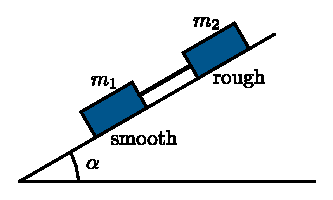
\includegraphics[width=4cm]{test}
\end{figure*}

Test for figure in list.
\begin{enumerate}
\item
One
\item
Two with figure.
\begin{figure*}
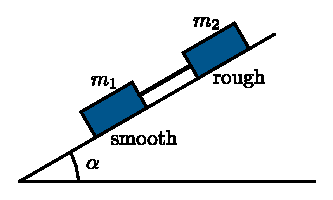
\includegraphics[width=4cm]{test}
\end{figure*}
\item
Three
\end{enumerate}

\lipsum[1]
\begin{marginfigure}
\caption{Figure test \label{fig-ex-test}}

\begin{tikzpicture}
\draw (0,0) -- (1,1);
\draw (1,0) -- (0,1);
\end{tikzpicture}
\end{marginfigure}
Test for wide figure.
\begin{widefigure*}
\begin{tikzpicture}
\draw[axis] (0,0) -- (15,0) node[xlab] {$x$};
\draw[axis] (0,-1.5) -- (0,1.5) node[ylab] {$y$};
\draw (0,0) sin (2,1) cos (4,0) sin (6,-1) cos (8,0) sin (10,1) node[above] {$y=\sin x$} cos (12,0) sin (14,-1);
\end{tikzpicture}
\end{widefigure*}


\lipsum[1]
\begin{marginfigure}
\caption{Figure test using includegraphics\label{fig-cross-marginfigure}}
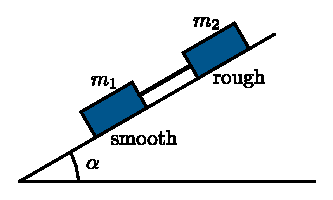
\includegraphics[width=4cm]{test}
\end{marginfigure}
\marginnote{This marginnote is placed in exactly the same place as the marginfigure --- notice how the first line exactly overlaps the end of the caption.}

\section{Theorems and proofs}
\begin{theorem}
\lipsum[133]
\end{theorem}
\begin{proof}
\lipsum[133]
\end{proof}
\begin{theorem}
\lipsum[133]
\end{theorem}
\begin{proof}[heading]
\lipsum[133]
\[
E=mc^2
\]
\end{proof}

For a named theorem use \verb”theorem*” to suppress the number.
\begin{theorem*}[Fundamental theorem of algebra]
Every polynomial of degree greater than one has a root in $\mathbb{C}$.
\end{theorem*}



\section{Nesting tests}

\begin{style2box}
\begin{activity}
\lipsum[133]
\begin{solution}
\lipsum[1]
\end{solution}
\end{activity}
\end{style2box}

\begin{style4box}
\begin{example}
\lipsum[133]
\begin{solution}
\lipsum[1]
\end{solution}
\end{example}
\end{style4box}

\begin{style4box}
\lipsum[133]
\begin{figure}
\caption{Figure test using Tikz. Note that commands in figure captions need to be robust like \hexagon{} and \(\mathbb{R}^2\).}
\begin{tikzpicture}
\draw[axis] (-0.5,0) -- (4,0) node[xlab]{$x$};
\draw[axis] (0,-0.5) -- (0,4) node[ylab]{$y$};
\draw[red,domain={0:3.5}] plot (\x,{(\x)^2/4}) node[black,right] {$y=x^2$};
\end{tikzpicture}
\end{figure}
\lipsum[133]
\end{style4box}

The following shows the optional title argument for a proof and also shows how to change the numbering of the steps if desired.
\begin{proof}[optional title]
%Do the following steps.
\begin{enumerate}[(a)]
\item foo 
\item bar
\end{enumerate}
\end{proof}

\section{Issues and workarounds}

The following shows how to format subexercises that have displayed aligned equations.
\begin{exercise}
For each of the following homomorphisms, determine \(\mathrm{Im}(\phi)\) and state whether \(\phi\) is onto.
\begin{enumerate}
\item \(\begin{array}[t]{r@{\,}l}
\phi:(\mathbb{Z},+)&\longrightarrow (\mathbb{Z}_{12},+_{12})\\
  n&\longmapsto n\pmod{12}
  \end{array}\)
\item \(\begin{array}[t]{r@{\,}l}
\phi:(\mathbb{Z},+)&\longrightarrow (\mathbb{R}^*,\times)\\
  n&\longmapsto 2^n
  \end{array}\)
\end{enumerate}
\begin{solution}
To be added.
\end{solution}
\end{exercise}

\paragraph{Issues}
\begin{enumerate}
\item
The moving solutions (namely the exercise and activity solutions) use the verbatim package to do the moving, which means that \verb”\end{solution}” must appear on a line on its own. This is not such a great problem as the error message is very specific if an author breaks this rule.
\item
The figure (and table) captions are currently fully justified, but should be ragged right.
\item
Any commands in a figure caption need to be robust. This is because they are written to a separate file to allow the possibility of producing a list of figures.
\item
If an overfull hbox occurs within a box then the box will expand to fit the contents. If a pagebreak occurs in the box then the box on the first page expands to fit even if the overfull hbox does not occur on this page. After the page break the box returns to its natural length, which can mean that content spills out to the right if there is an overfull hbox on the page. The solution is to fix the overfull hbox's.
\item
If a marginfigure environment appears in the middle of a sentence then it will absorb the space following so that the words either side of the marginfigure will coalesce. The work-around is to place marginfigures at the beginning of a paragraph.

\end{enumerate}

\paragraph{To Do}
\begin{enumerate}
\item
\verb”sourceref”
\item
Glossary items.
\item
Add mechanism for defining new icons. (and a better error message if an icon is not defined.)
\item
Add environments for structured content XML elements that are not used on paper (e.g. 
\verb"mediacontent").
\end{enumerate}

\printexercisesolutions
\printactivitysolutions
\printindex
 
\end{document}